\documentclass[12pt,a4paper]{report}

\usepackage[utf8x]{inputenc}
\usepackage{amsmath}
\usepackage{amsfonts}
\usepackage{amssymb}
\usepackage{graphicx}
\usepackage{enumitem}
\usepackage{fontspec}
\usepackage{pgf}
\usepackage{tikz}
\usepackage{calrsfs}
\usepackage{ifthen}
\usepackage{algpseudocode}
\usepackage{cancel}	
\usetikzlibrary{arrows, matrix}

\begin{document}

\begin{titlepage}
	\centering
	{\scshape\LARGE Universidad Nacional Autónoma de México \par}
	\vspace{1cm}
	{\scshape\Large Computación Distribuida\par}
	\vspace{1.5cm}
	{\huge\bfseries Tarea 3\par}
	\vspace{.5cm}
	{\Large\itshape Edgar Quiroz Castañeda \par}
    \vspace{.5cm}
	{\Large\itshape Jerónimo Almeida Rodríguez \par}
	\vfill
	 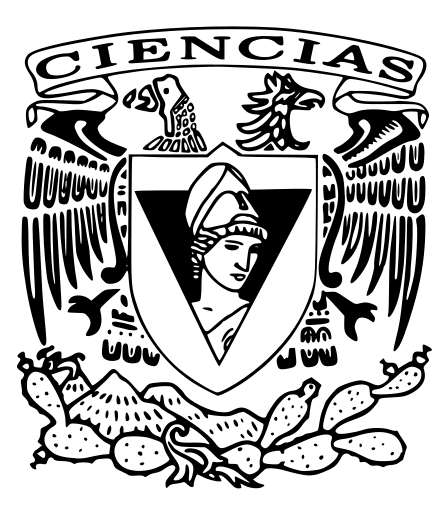
\includegraphics[width=0.5\textwidth]{escudo_f-ciencias.png}
	\vfill

% Bottom of the page
	{\large Jueves 20 de septiembre del 2018 \par}
\end{titlepage}

\pagebreak
\setlength{\voffset}{-0.75in}
\setlength{\headsep}{5pt}


\begin{enumerate}
	%Ejercicio 1
	\item {
		Considere el siguiente algoritmo para resolver el consense en un sistema
		con $n$ procesos y con a lo más $f$ procesos fallidos.\\
		\[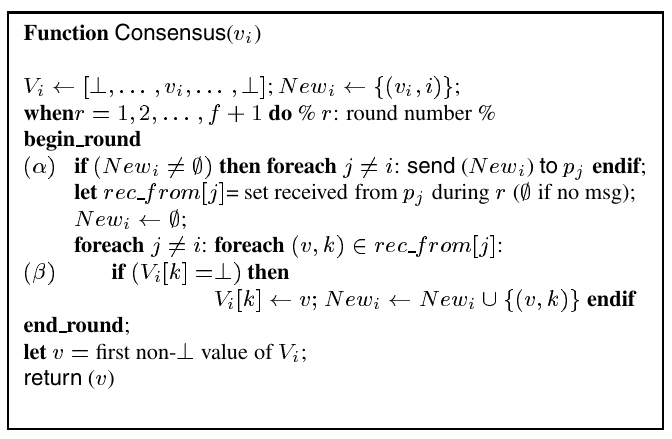
\includegraphics[width=0.5\textwidth]{consensus.png}\]

		\begin{enumerate} [label = \alph*)]
			\item {
				Argumenta por qué es necesario ejecutar $f+1$ rondas para llegar a un acuedo.\\

				Los errores del modelo son únicamente de tipo crash, esto es que una vez fallado
				proceso no vuelve a funcionar.\\
				Esto significa que la cantidad de procesos vivos se queda igual o disminuye.
				Y cómo los procesos son donde está guardad la información, entonces la
				información que se puede obtener en cada ronda se queda igual o disminuye.\\
				Entonces, si en una ronda no muere ningún proceso, todos los procesos obtendrán
				toda la información disponible, y en cualquier ronda posterior habrá igual o
				menos información disponible.

				Notemos que si uno o varios procesos mueren antes de enviar cualquier
				tipo de información, entonces la información nueva que tenían se pierde.\\
				Si eran los únicos procesos vivos que tenían esa información, entonces esa
				información se puede ignorar, pues al no tenerla nadie es como si nunca
				hubiera existido. \\
				Si la información la tiene otro proceso que no ha muerto,
				entonces durante esa misma ronda el otro proceso habrá enviado esa información
				a todos los demás.\\
				De cualquier manera, la muerte de los procesos no causa inconsistencias en
				el resultado final, pues todos siguen recibiendo la misma información.\\
				Lo que puede causar inconsistencia en la decisión, es que un proceso
				muera mientras está enviando información que sólo ese proceso tiene.\\
				Esto pasa porque parte de los procesos tienen información que la otra
				parte no tiene.\\

				Entonces siempre y cuando haya una ronda donde algún proceso muera antes
				de enviar algo o nunca muera, entonces al final todos los procesos obtendrán
				la misma información, por lo que se llega a un consenso.\\
				Entonces en el caso extremo en cada ronda mueren procesos mientras están
				enviando infrmación, y el caso que requiere más rondas es cuando exactamente
				un proceso muere de esta manera cada ronda.\\
				Entonces después de $f$ rondas es posible que en cada ronda
				un proceso con nueva información haya muerto mientras enviaba la información
				a otro proceso, por lo que algunos procesos tendrían más información que otros.\\
				Como ya murieron $f$ procesos, entonces ya no puede moriri más procesos.
				Al realizar otra ronda, aseguramos que en esa ronda ningún proceso
				va a morir, y todos lor procesos vivos obtendrán toda la información
				disponible es esa ronda. Entonce todos tendrán la misma información y
				podrán llegar a un consenso.\\
			}
			\item{
				Modifica el algoritmo de la figura 1 para resolver el consenso en
				$min(t+2, f+1)$ donde $t$ es la cantidad de procesos que fallan en la
				ejecución.\\

				Del inciso anterior se sabe que si en una ronda ningún proceso muere,
				entonces todos los procesos vivos van a tener toda la información
				disponible por lo que queda de la ejecución. Entonces es posible llegar
				a un consenso en ese punto.\\
				De forma más restringida pero análoga, si en una ronda todos los procesos
				envían información a un cierto proceso, entonces este proceso ya sabe
				todo lo que puede saber.\\
				Pero ¿cómo se puede saber en qué ronda ningún proceos muere?\\
				Una solución simple es que todos los procesos en todas las rondas envíen
				algo como señal de que siguen vivos, y que todos los procesos lleven
				un registro de los procesos de los que reciben una señal de vida en cada ronda.
				Entonces, si en una ronda la cantidad de procesos que responden a cierto proceso
				es la misma que en la ronda anterior, el proceso ya sabe todo
				lo que puede saber en esa ronda.\\
				Pero puede pasar que alguno de los procesos que le enviaron información
				mueran antes de enviarla a todos, por lo que faltaría reenviar una
				última vez la información nueva que tiene a todos los demás. Entonces ya
				puede garantizar que todos ya saben todo lo que puedes saber.\\
				Y se puede llegar a un consenso en potencialmente menos de $f+1$ rondas
				si en la ejecución hay menos de $f$ procesos muertos.
				De forma análoga a la anterior, el caso donde más rondas se ejecutan es
				cuando en cada ronda un proceso muere justo a media ejecución. Entonces,
				al acabar la ronda $t$, ningún proceso más va a morir.\\
				En la ronda $t+1$ todos los procesos se dan cuanta de que ya saben todo
				lo que puede saber. Entonces envían su información nueva y en la ronda
				$t+2$ toman su elección de valor final, que como todos tiene la misma
				información, es la misma elección para todos.\\
				La moficación consisa sería en la línea $(\alpha)$ quitar la condición,
				para que en todas las rondas se envía algo, se tenga información nueva o no.\\
				Y también hay que agregar un registro de los procesos que hay respondido.\\
				Esto sería algo cómo
				\\\\$R(r) \leftarrow$ set of clients answering during the $r$ round\\\\
				en la línea después de la $(\alpha)$.\\
				Y también hay que agregar algo justo al final de la ejecución de la ronda
				donde se compara $R(r)$ y $R(r-1)$. Por comodidad digamos que $R(0) = \Pi \setminus \{i\}$.
				Si son iguales, entonces ya se sabe
				todo lo que se puede saber, y después de enviar toda la información nueva
				durante la siguiente ronda, se puede decidir un valor.\\

				Como la cantidad de ejecuciones sigues siendo a lo más $f+1$, entonces
				el algoritmo termina. Cómo aun se sigue escongiendo la primera entrada
				no nula del arreglo de información, entonces se escoge alguno de los valores
				entrada, por lo que sigue siendo válido.\\
				Por el razonamiento anterior, al acabar las $t+2$ o $f+1$ rondas, todos
				los procesos vivos tienen la misma información, por lo que al decidir
				el valor final, todo decidirán lo mismo, por lo que el algoritmo el correcto.
				Si $t = f$, entonces la cantidad de rondas acaba en $f+1$
				como en el algoritmo original. Si $t \l f$, entonces acaba en las $t+2$
				rondas descritas anteriormente.
				Entonces se ejecutan $min(t+2, f+1)$ rondas.

			}
			\item{
				Muestra una ejecución para 4 procesos donde se ejecutan el máximo de
				rondas del algoritmo propuesto.\\

				Esto corresponde a la ejecución donde en cada ronda falla exactamente un
				proceoso a la mitad de la ejecución. Para que haya algún proceso al final
				que decida, debe de pasar que $f$ sea a lo más la cantida de procesos menos 1.
				Entonces, en este caso digamos que pueden fallar 3 procesos.

				Al iniciar la ronda 1 tenemos que
				\begin{center}
					\begin{tabular}{|c|c|}
						\hline
						Proceso & Información\\
						\hline
						1 & $\{v_1, \bot, \bot, \bot\}$\\
						\hline
						2 & $\{\bot, v_2, \bot, \bot\}$\\
						\hline
						3 & $\{\bot, \bot, v_3, \bot\}$\\
						\hline
						4 & $\{\bot, \bot, \bot, v_4\}$\\
						\hline
					\end{tabular}
				\end{center}
				Luego digamos que el proceso 1 muere después de enviar la información a
				2, por lo que no llega a 3 ni a 4.  Inicialmente todos lo procesos
				tenían que $|R(0)| = 3$. Al acabar la ronda 1, 2 tiene que $|R(1) = 3|$, por
				lo acuerda que después de enviar toda su información la próxima ronda,
				va a decidir.
				Los demás tienen que $|R(1) = 2|$, por lo que siguen su ejecución sin cambios.
				Entonces al iniciar la ronda 2 tenemos
				que
				\begin{center}
					\begin{tabular}{|c|c|}
						\hline
						Proceso & Información\\
						\hline
						\cancel{1} & $\cancel{\{v_1, \bot, \bot, \bot\}}$\\
						\hline
						2 & $\{v_1, v_2, v_3, v_4\}$\\
						\hline
						3 & $\{\bot, v_2, v_3, v_4\}$\\
						\hline
						4 & $\{\bot, v_2, v_3, v_4\}$\\
						\hline
					\end{tabular}
				\end{center}
				Siguiendo el patrón, digamos que el proceso 2 muere después de enviar
				información a 3, por lo que 4 nunca la recibe. Cómo 2 nunca termina de
				enviar su información, entonces nunca decide. Para 3 tenemos que
				$R(2) = 2$, por lo que sabe que ya tiene toda la información, por lo que
				dará su decisión después de enviar toda su información nueva la siguiente
				ronda. Para 4 $P(2)=1$.\\

				Al iniciar la ronda 3 tenemos
				\begin{center}
					\begin{tabular}{|c|c|}
						\hline
						Proceso & Información\\
						\hline
						\cancel{1} & $\cancel{\{v_1, \bot, \bot, \bot\}}$\\
						\hline
						\cancel{2}& $\cancel{\{v_1, v_2, v_3, v_4\}}$\\
						\hline
						3 & $\{v_1, v_2, v_3, v_4\}$\\
						\hline
						4 & $\{\bot, v_2, v_3, v_4\}$\\
						\hline
					\end{tabular}
				\end{center}

				Y ahora 3 muere justo después de enviar su mensaje a 4.
				Tenemos que para 4 $R(3) = 1$, por lo que 4 ya sabe todo, y después
				de enviar toda su información la próxima ronda, decidirá.

				Al iniciar la ronda 4 tenemos que

				\begin{center}
					\begin{tabular}{|c|c|}
						\hline
						Proceso & Información\\
						\hline
						\cancel{1} & $\cancel{\{v_1, \bot, \bot, \bot\}}$\\
						\hline
						\cancel{2}& $\cancel{\{v_1, v_2, v_3, v_4\}}$\\
						\hline
						\cancel{3} & $\cancel{\{v_1, v_2, v_3, v_4\}}$\\
						\hline
						4 & $\{v_1, v_2, v_3, v_4\}$\\
						\hline
					\end{tabular}
				\end{center}
				4 envían lo que sabe, aunque nadie lo recibe. Al final de la ronda 4
				el estado global entonces es el mismo que al inicio.
				Y como ya pasaron las 3+1 = 4 rondas, entonces los procesos vivos, que
				solo es 4, deciden el valor, que en este caso es $v_1$.
				Cómo solo un proceso quedó vivo, entonces la ejecución es correcta.\\
			}
			\item{
				Muestra una ejecución para 4 procesos donde se ejecuten el mínimo de
				rondas del algoritmo propuesto.\\
				La forma más sencilla de mostrar esto sería con una ejecución sin ningún
				error, por lo que terminaría en 0+2 = 2 rondas.\\

				Todos los procesos inician con $R(0) = 4 - 1 = 3$.\\
				Al inicio de la primera ronda tenemos que
				\begin{center}
					\begin{tabular}{|c|c|}
						\hline
						Proceso & Información\\
						\hline
						1 & $\{v_1, \bot, \bot, \bot\}$\\
						\hline
						2 & $\{\bot, v_2, \bot, \bot\}$\\
						\hline
						3 & $\{\bot, \bot, v_3, \bot\}$\\
						\hline
						4 & $\{\bot, \bot, \bot, v_4\}$\\
						\hline
					\end{tabular}
				\end{center}

				Todos los procesos viven. Todos los procesos tienen $R(1) = 3$, pues
				recibieron mensajes de todos. Todos los procesos entonces saben que
				ya tienen toda la información. Entonces después de enviarla la siguiente
				ronda, van a decidir el valor final.\\

				Al inicio de la segunda ronda tenemos que

				\begin{center}
					\begin{tabular}{|c|c|}
						\hline
						Proceso & Información\\
						\hline
						1 & $\{v_1, v, v_3, v_4\}$\\
						\hline
						2 & $\{v_1, v, v_3, v_4\}$\\
						\hline
						3 & $\{v_1, v, v_3, v_4\}$\\
						\hline
						4 & $\{v_1, v, v_3, v_4\}$\\
						\hline
					\end{tabular}
				\end{center}
				Entoces, después de enviar su información nueva, ningún proceso cambia
				la información que tiene, pues ya saben todo.\\
				Cómo ya lo tenían planeado cada uno independientemente, deciden su valor
				final. En todos los casos es $v_1$, por lo que la ejecución es correcta.\\
			}
		\end{enumerate}

	}




	%Ejercicio 2
	\item {
		Sean $A$ y $B$ dos procesos conectados por dos canales unidireccionales.
		La secuencia $G_t$ en el tiempo $t$ corresponde a $m_1, ..., m_k, n_1, ..., n_l$
		donde los $m_i$ corresponden a los mensajes enviados de $A$ hacia $B$ y $n_i$
		los enviados de $B$ a $A$, donde $k_1$ es el mensaje más reciente enviado
		por el canal.

		\begin{enumerate} [label = \alph*]
			\item {
				¿Qué cadenas de bits no son válidas al ejecutar el protocolo?\\
				Las cadenas que no son válidas en el protocolo son aquellas que:
				\begin{enumerate}
					\item[i]{
						Por la manera en la que está definido el algoritmo, tenemos que
						ninguna cadena puede iniciar con $1$.
					}
					\item[ii]{
						Tampoco puede haber alguna cadena en la que haya más de un cambio en la
						 coloración, por ejemplo $001100$.\\
						Esta cadena no es válida porque, según el algoritmo, $A$ no cambia de 
						valor hasta que que recibe un bit de $B$ con el valor que le está 
						enviando. Entonces, $A$ está enviando un mensaje con un valor, $B$ lo 
						recibe y $B$ lo retransmite ese bit. Mientras tanto, no hay cambios 
						todavía en el valor que $A$ está transmitiendo. Hasta este punto, si es 
						la priemra iteración, la cadena tiene un mismo color. Cuando $A$ recibe 
						el bit con el color que le está enviando $B$, cambia su valor y empieza a 
						transmitirlo. En este punto hay dos colores en la gráfica: el nuevo valor 
						que transmite $A$ y el valor anterior que estaba transmitiendo $A$ y que 
						ahora transmite $B$. Si iteramos sobre este proceso, podemos observar que 
						solamente hay dos colores en la gráfica en cualquier momento mientras se 
						esté ejecutando el algoritmo.
					}
					\item[iii]{
						La longitud de bits de un mismo color solamente es menor a dos cuando es 
						el primer bit en una cadena después de un cambio de coloración o el 
						último bit de confirmación de un mensaje. De otro modo la cadena no es 
						válida.\\
						Sabemos por el inciso anterior que solamente puede haber dos colores en 
						la cadena en cualquier momento dado. Esto significa que $A$ no cambia su
						valor mientras que no reciba de $B$ un bit con el color que está 
						transmitiendo. Entonces, para el primer caso, si es el primer bit 
						transmitido en la ejecución del algoritmo, la longitud de la cadena es 1 
						y solamente hay un color en la cadena. El bit que le sucede 
						inmediatamente tiene el mismo valor porque $B$ recibió y transmitió el 
						bit recibido de $A$ antes de que $A$ pudiera enviar un siguiente mensaje
						o $A$ volvió a transmitir un mensaje con el mismo bit. Observando ahora 
						el segundo caso vemos que $B$ está transmitiendo los valores que recibe 
						de $A$. Entonces, una vez que $B$ envió el mensaje y lo retransmitió a 
						$A$, va a seguir recibiendo ese mismo valor de $A$ hasta que $A$ reciba
						el bit que le está enviando a $B$. Entonces, tenemos que el valor de la 
						cadena se va recorriendo mientras $B$ transmite y $A$ recibe. De esta 
						manera podemos observar que los bits del canal de $A$ a $B$ no cambian 
						mientras que los bits de $B$ a $A$ van recorriendo el valor hasta que 
						solamente queda un bit de valor distinto antes de llegar a $A$ y se 
						cumple la propiedad anterior que solamente hay un cambio de color en la 
						cadena en cualquier momento de la ejecución del algoritmo. En el momento 
						en el que $A$ recibe este bit, la cadena es de un mismo color y 
						regresamos a un caso inicial.\\
						Cómo el proceso no crea mensajes podemos asegurar que no va a haber un 
						bit solo de color distinto en la cadena excepto por los casos mencionados
						anteriormente.
					}
				\end{enumerate}
			}
			\item{
				¿Cuándo hay un cambio de bits en la coloración?\\
				Hay un cambio en la coloración cuando $A$ recibe un mensaje de $B$ con el bit que
				está transmitiendo, cómo lo vimos en el el inciso $2.a.ii$.
			}
			\item{
				Ejecuta el protocolo de forma que en la coloración hayan al menos 4 unos.
				El estado en el que la coloración tenga al menos cuatro unos se da solamente en 
				el momento antes de que $A$ reciba la confirmación de $B$ en una ronda par y si
				los canales son suficientemente lentos para que en cualquier momento dado haya al 
				menos dos mensajes en el canal sin tomar en cuenta los mensajes perdidos. \\
				\begin{tikzpicture}
  \matrix (m) [matrix of math nodes,row sep=3em,column sep=4em,minimum width=2em]
  {
     1 & 1 \\
     1 & 1 \\};
  \path[-stealth]
    (m-1-1) edge node [left] {$A$} (m-2-1)
            edge node [below] {$...$} (m-1-2)
    (m-2-2) edge node [below] {$...$} (m-2-1)
    (m-1-2) edge node [right] {$B$} (m-2-2);
\end{tikzpicture}
				
			}
		\end{enumerate}

	}

	\item{
		Escribe un resumen de la clase y plática impartidas por Michel Raynal.

		"God made bits, everything else is the work of man" -Michel Raynal\\
		La informática es el área de estudio dedicada al estudio de que es computable
		o no. Es decir que se puede lograr siguiendo una serie determinada finita de pasos.\\
		Esto incluye todo lo relacionado con algoritmos y computabilidad.\\
		También se puede ver como la formalización matemática de la tecnología.\\
		Dentro de esto, vive el área de los sistemas distribuidos, que involucran
		a varios procesos, máquinas de Turing, independientes que se comunican de
		alguna manera que puede ser memoria compartida (computación concurrrente)
		o mensajes por un canal de comunicación.\\
		A difenrencia de la computación en paralelo, la independecnia de los procesos
		es algo impuesto más que una elección de diseño, en donde no se conoce el
		estado global del sistema y todas las decisiones son locales.\\
		Con esta definición puede haber una gran cantidad de configuraciones, como
		la dirección de los canales de comunicación, el tipo de errores de canal o errores
		de procesos, la gráfica asociada a todos los proceosos con los canales de comunicación,
		o la sincronía de la comunicación.\\
		Los errores de proceso pueden ser de tipo "crash", donde cuando un proceso
		falla nunca se vuelve a recuperar, o bizantinos, cuando un proceso tiene un
		comportamiento no predecible.\\
		Los errores de cnal pueden ser de pérdida de mensajes, de intercambio de mensajes
		o de modificación de mensajes.\\
		En todo los casos, cada procesos tiene tres estados: enviar, recibir y ejecutar.
		En un modelo síncrono, se tiene que todas las acciones se ejecutan siguiendo
		un reloj global. Se puede garantizar que si un mensaje no llega en ciertos ciclos,
		entonces nunca va a llegar.\\
		Mientras que en un modelo asíncrono las acciones se ejecutan después de la llegada
		de algún mensaje, y no hay garantía sobre cunado algo va a llegar.\\
		Hay dos grandes problemas.\\
		Luego ¿cómo se define un problema en estos modelos?
		Deben de tener dos propiedades que su solución debe de cumplir, que son
		"safety" que es una restricción sobre lo que no debe de pasar, y "liveness" que es
		una manera de asegurar que se tiene que realizar algo.
		Entonces una solución es un algoritmo tal que existe una demostración que
		prueba que el algoritmo cumples esas dos propiedades para cualquier posible
		ejecución del algoritmo.\\
		En general, en un modelo sin errores, todo problema es relativamente sencillo
		de resolver. Por lo que en general se busca el modelo con más errores donde
		aun es posible resolver un problema.
		Hay dos problemas en especial que se vieron durante la plática.
		El primero es el ataque coordinado.

		El otro es el problema del consenso

	}

\end{enumerate}
\end{document}
